\documentclass{standalone}
\usepackage{tikz}
\begin{document}


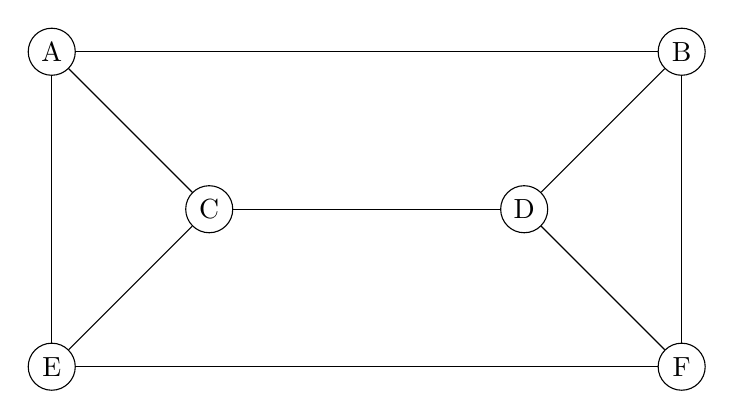
\begin{tikzpicture}[scale=2]
\tikzstyle{vertex}=[circle, draw, minimum size=17pt, inner sep=0pt]
\node[vertex] (A) at (0,2) {A};
\node[vertex] (B) at (4,2) {B};
\node[vertex] (C) at (1,1) {C};
\node[vertex] (D) at (3,1) {D};
\node[vertex] (E) at (0,0) {E};
\node[vertex] (F) at (4,0) {F};

\path 
(A) edge (B)
    edge (C)
    edge (E)
(B) edge (D)
    edge (F)
(C) edge (D)
    edge (E)
(D) edge (F)
(E) edge (F);

\end{tikzpicture}

\end{document}
